\section{Meetings and Proceedings}
In this section, we detail exactly what happened at select meetings, whose events bear particular significance over the development of our robot.

\subsection{Preseason Overview -- Meeting 1: 2013-08-31}
We held a preseason meeting in order to go over scheduling, recruitment of new members, and hold a quick review of what we learned from our last season. One of the main items we discussed was our scheduling, and as a team we decided to take an aggressive approach towards our first couple of regional competitions in order to secure a place in St. Louis. Because of this, we may need to cut back on scoring the maximum number of points and instead focus on scoring a high, yet consistent number of points. We found out that we need to secure our electronics and work with the field control issues that we were issues. We also plan on placing a much larger emphasis on the CAD design of our robot than we have in our two previous years as it is an efficient way to quickly discover and troubleshoot problems prior to building the system. 

Our final goal is to have two weeks of drive practice before our first regional on December 14th, important for both driver and coaches, to figure out the timing of the game, as well as things that we can or cannot do in game. Organization of the team this year will be facilitated through the use of Google Groups, which will allow all the team members and their parents to be easily contacted for meetings, and will hopefully foster some discussion over build design or game strategy. 

We also decided to meet a few hours after the game was released next week so team members could think about strategies ahead of time and add to the strategy discussion of our first meeting of the season. The meeting was fairly short, but got the team in the right mindset for the upcoming season, and got everyone excited for the  new season!

\newpage \subsection{Initial Design -- Meeting 2: 2013-09-07}
The team decided last week to meet a few hours after the game video and rules were released, so by the time our meeting started, everyone had an idea of how they thought the robot should work, and be built. Fortunately, most team members were on the same page and wanted to focus on scoring as many blocks into the baskets as possible, in a manner that would allow for a integration in the lifting and scoring mechanism. We decided to focus on every aspect of the game for our qualifiers, since it seems like we could consolidate all of the mechanisms into very few.

After a fairly long strategy discussion, some ideas were thrown around as to how to pick up and score the blocks, since we always have a difficult time getting our game pieces, and a rough idea of a mechanism was developed that would use a roller system and a block hopper that would pick up and score the blocks. There is still significant discussion considering the way we will go about constructing a lifting mechanism, with different arguments for and against a rotating arm and a more standard but perhaps less efficient forklift, similar to ``Ring It Up!''. Some of our team members have some experience with constructing forklifts from prior FTC seasons, so we have some idea of what kind of issues we might come across with that kind of design. One thing we discussed was making sure we construct and purchase our materials with a little more regard for quality than we have in previous years, but we wanted to focus on simplicity this season as it worked out very well for us three years ago, and the ideas we are thinking of currently all seem to fit this idea.

Members of the team have assumed different jobs to complete before the next meeting, such as researching lifting mechanisms, getting a BOM for the field and purchasing the materials, and researching the specifications of an IR beacon and sensor, since the team also decided that scoring the block during autonomous is absolutely imperative to the outcome of this game. It is essentially free points that even a defensive robot cannot stop. As of right now we are choosing to focus the endgame period, since lifting and raising the flag are relatively simple tasks. 

We are considering purchasing the AndyMark field, as it would provide us a standardized field and a better replication of the interaction of the robot with the field during competition. 

\newpage \subsection{General Design -- Meeting 3: 2013-09-14}
Today was our second main meeting; we discussed several different raising mechanisms, since we as a team have decided that it was the most important system of our robot.

Our main idea for lifting is an arm that is centered around the top corner. We are designing it to be just long enough to allow us to climb the bar as well as to clear the front block scooper. As for the material, we were looking at Delrin, and wood for our prototype. Delrin has incredible tensile strength. If a material is homogeneous then the tensile and flexural strengths are identical. However, most materials have defects in them which act to concentrate the stresses locally, which in turn cause a localized weakness. We have determined that the flexural strength is greater in the Delrin over the wood as follows. We first see that method for calculating flexural strength is: \[\sigma = \frac{3FL}{2bd^2}\] and we are looking to see which sheet can take in the maximum force, $F$. It directly follows that as we increase $b$, the width measured in in, and $d$, the  thickness measured in in, the sheet can withstand a greater force. Elementary analysis allows us to see that the Delrin is superior than the wood. This will assure us that if our wood prototype works, so should our final design. It will also be able to withstand in competition. 

For the flag spinner, we discussed using some external pins or some type of rubber-esque substance to push against the edge and raise it up. We believe that a rubber-esque material will work. We plan on using 3 NXT motors to provide enough torque and speed to raise the flag. Our goal is to raise the flag in under 5 seconds. 

We also spent a lot of time discussing the importance of autonomous and the structure of our code. We are looking at dynamic autonomous programs that are able to dodge other robots if need be. We are looking forward to prototyping within the next several weeks. Our meetings have mainly comprised of theorizing about code and 3D modeling our robot. We are sharing with the younger students much of the knowledge we have learned over the years as well. 

\newpage \subsection{Initial Field Build -- Meeting 4: 2013-09-21}
Today we began building the field, discussed the lifting, got mail, worked on autonomous theory, cut PVC with safety glasses, and had some fun moving our very mobile robot for a while.  In the mail we received one half of the blocks necessary for the field.
For building we:
\begin{enumerate}
\item Painted the wood
\item Cut all the pvc pipes for the flag spinner
\item Wore safety glasses
\item Cleaned up a lot of pvc dust
\item Screwed temporary screws to the flanges onto the wood
\end{enumerate}

Flag Spinner:
\begin{itemize}
\item Involves NXT motors
\item Gearing 6:1
\item Rubber-esque material did not work out
\item Using extruding pins
\end{itemize}

\newpage \subsection{First Prototype -- Meeting 5: 2013-09-28}
Today was a day for laying out drawings, finalizing designs, and testing some of the flag spinner prototypes. 

We started the day with the usual bit of socialization, before returning to work. The primary topic of discussion is the acquisition mechanism for the blocks. It has been speculated up until this point that we are going to be using a roller, and it looks like those plans may come to fruition. 
We received several items today, including some Tetrix motors, as well as M3 screws and the other half of the blocks.

A to-scale side view drawing shows that the arm we want to design and guiding channels will take up about 7 inches on either side, leaving 8 inches in the middle to mount the block grabbing mechanism on. This fits within our expectations.

It is worth noting that the since we are designing the robot out of raw materials we are using metric, as opposed to the imperial u-channels, so there is some difficulty in lining up the holes if we plan to use any Tetrix. This is a prototype however, and the arm we plan to design for the final design would be out of Delrin, and can be designed to fit our needs. The prototype wooden arm also has potential tolerance issues. There is about a 1 block tolerance on the size of the spinning blocks. Stability is key. 

We constructed our first prototype, we assembled the outside arms from plywood. From left to right, there are two arm chassis pieces, the arm pieces and then two arm chassis pieces. The frame design is an A-frame and it works pretty well.

\begin{figure}[H]
\begin{center}
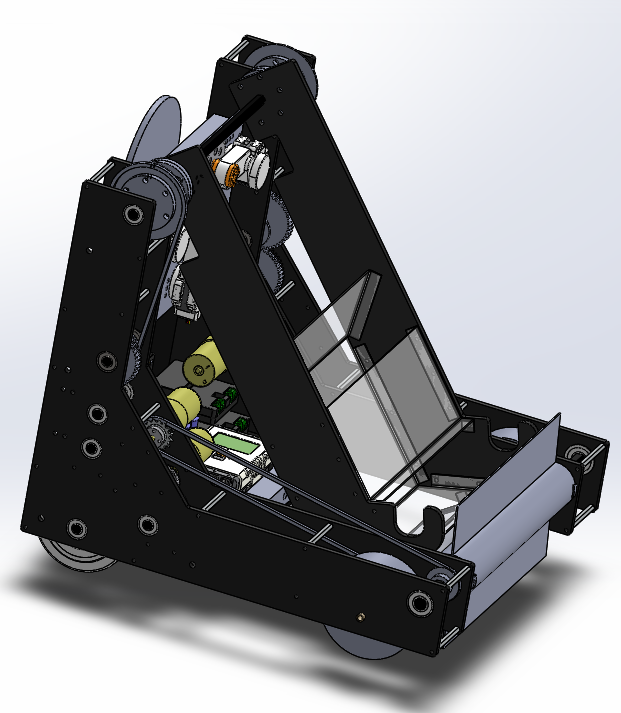
\includegraphics[scale=0.5]{images/RobotV1.png}
\end{center}
\caption{This is the first revision of our Solidworks. We can see the block acquisition device that is essentially a roller that will inhale blocks into our robot}
\end{figure}

Force is not an issue, and remains at a 16:1 ratio with torque gained. It is important to note that the force DOES double when an additional layer is added, however, with the 16:1 ratio between the movement of the bars, the speed with which the bars are raised ALSO doubles. This means that, though the force doubles, the speed at which the arm go up is also doubled. That implies that any torque issue created by adding another layer to the mechanism can be resolved by multiplying the gear ratio of the chain motor by two. The same vertical speed will be achieved.
The prototype is very functional. We connected it to the (makeshift) motor, and ran it. The mechanism lifted very well. The following problems were noted:
\begin{itemize}
\item Block pickup does not work
\item Lifting does not lock after power is lost
\item The wooden shaft collars strip
\item It does not move fast enough
\item It makes the robot very back heavy
\end{itemize}

Possible solutions to these problems (in order) are:
\begin{itemize}
\item Switch from the roller
\item Jam the gears
\item Change the wood to metal
\item Add steel to the front
\end{itemize}

Despite these issues, the lifting mechanism works well, and glides smoothly as long as they aren't stripped. Granted it is currently in prototype form, the final version (which will be produced much more carefully), should be very effective.

We are currently looking into redesigning the block pickup mechanism as it does not seem to be effective. We plan on lowering the roller to the ground and seeing what happens. 

Currently, our projected maximum height is 32”, just over what we need to hang on the bar.

\newpage \subsection{Flag Spinner Initial Test -- Meeting 6: 2013-10-6}
Today's meeting was short - it was only two hours. We had a couple ideas we wanted to test, and the tests were successful. We verified our idea would work, and redrew the pictures from two days ago.

The idea we were testing today was whether or not we could raise the flag by using a rubber-like substance to mesh within it and spin. We soon saw that the NXT motors were not as powerful as we would like and the force that the rubber plate was inducing was off center. This makes it unfeasible to use. 

\begin{figure}[H]
\begin{center}
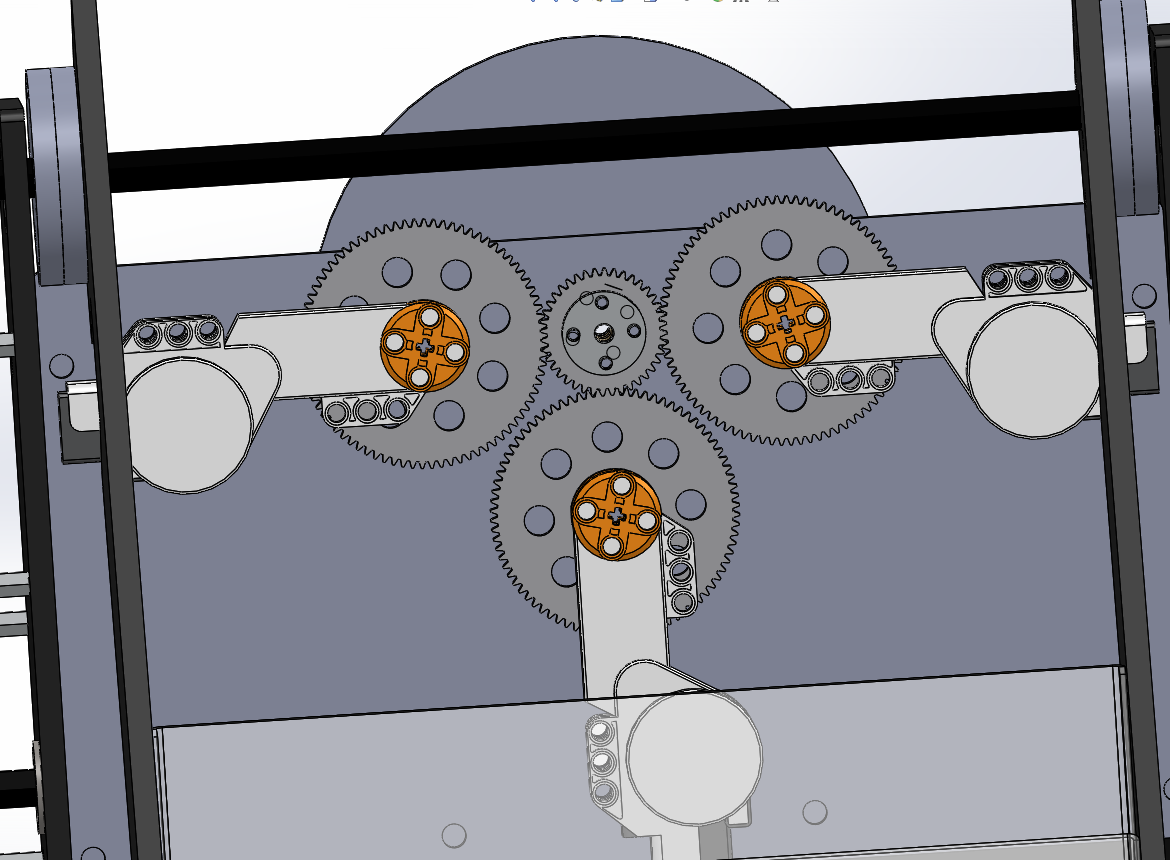
\includegraphics[scale=0.25]{images/FlagSpinnerV1.png}
\end{center}
\end{figure}


We plan on switching to the seemingly common extruded pins design. We plan on having two pins attached off center that are $180^\circ$ apart. We also plan on switching to a Tetrix motor with a $6:1$ gearing ratio. With this ratio, we will be able to raise the flag, theoretically, in under 10 seconds. 

However, this method adds an extra $1.5''$ to our length. As we must stay within the $18''$ length constraint, we may have to shorten our roller (block pickup mechanism). This may become problematic, but as far as we can see we should be able to work around it. 

For the pins, we had two ideas: the first is to use cut Tetrix axles. The second is to use longer Tetrix screws. We plan on using the Tetrix screws first to test and we may end up keeping them on afterwards. 

We also did some more testing with the roller. We experimented with lowering it and shrinking the radius of the aluminum tube. We chose a smaller inner radius due to the fact that it would weigh less and it would be easier to place near the ground. We are still running into issues of picking up much more than 4 blocks at a time. 

We decided on mounting it 1.5'' above the ground because this is just enough to let the blocks slide under as we roll. 

It is the popular idea that we want to completely redesign the block grabbing mechanism due to its inability to give us the accuracy and visibility that we want. Visibility is an issue when we go to the opposite side of the field. 

\newpage \subsection{Block Acquisition Redesign -- Meeting 7: 2013-10-11}
We have spent a lot of time working on scoring blocks, but we overlooked the difficulty of acquiring them. We decided to spend the day looking over our acquisition device as we found it was not very effective. We are looking into changing the roller into a much lower roller made of rubber. We are also looking into changing the entire design altogether. The main ideas consist of driving into blocks and then flipping them into our arm. However, many members of the team do not like the idea of multiple moving parts. 

We decided to extend the final aspect of the roller and found that it was completely ineffective. There is currently no member that continuously supports this idea. 

Today, Garrison proposed that we use a bulldozer like system. A flat plate that we would use to ram into the blocks. Essentially extending our arm to be outside of the frame. We built a first prototype with this and it seems to show some promise. We are still unsure of the implications that this has for the a final working idea. 

Another issue we see with this mechanism is that it is very easy for blocks to slip outside of our robot. 

We currently plan to go home and think about better ideas. We will probably have an in-depth Skype conversation over this idea. We look forward to improving this design as it needs a lot of work. 

The flag spinner was also entirely redesigned as follows:

\begin{figure}[H]
\begin{center}
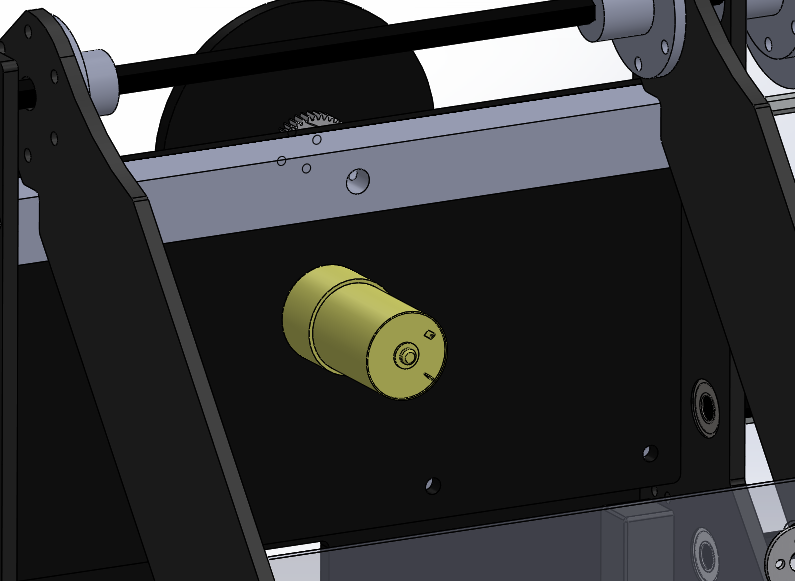
\includegraphics[scale=0.4]{images/FlagSpinnerV2Back.png}
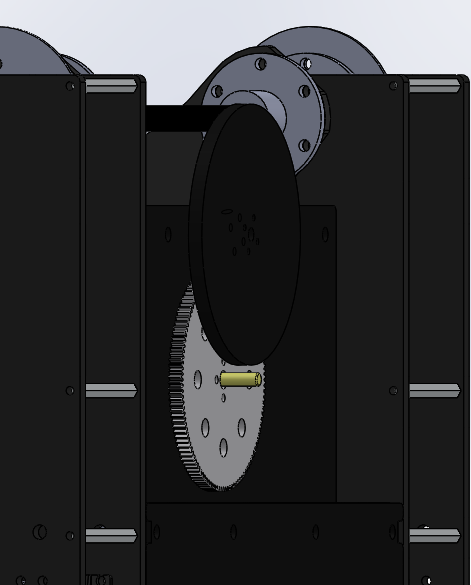
\includegraphics[scale=0.5]{images/FlagSpinnerV2Front.png}
\end{center}
\caption{Here we can see both sides of the new, redesigned, flag spinner. The notable changes include the switch to the Tetrix motor and the removal of the rubber backing in turn for extruding pins (not shown above).}
\end{figure}

\newpage \subsection{SolidWorks Redesign -- Meeting 8: 2013-10-18}
After coming back with new ideas, we spent the first hour of our meeting discussing the pros and cons of our new block acquisition mechanism. We all feel that a flat sheet on the ground that we can use to run into the blocks as a bulldozer is the optimal solution. 

We are designing it to be fully flush with the ground. We look forward to testing this out. In SolidWorks we are redesigning the base of the robot to be shorter to allow the bulldozer system to lie in front. 

\begin{figure}[h]
\begin{center}
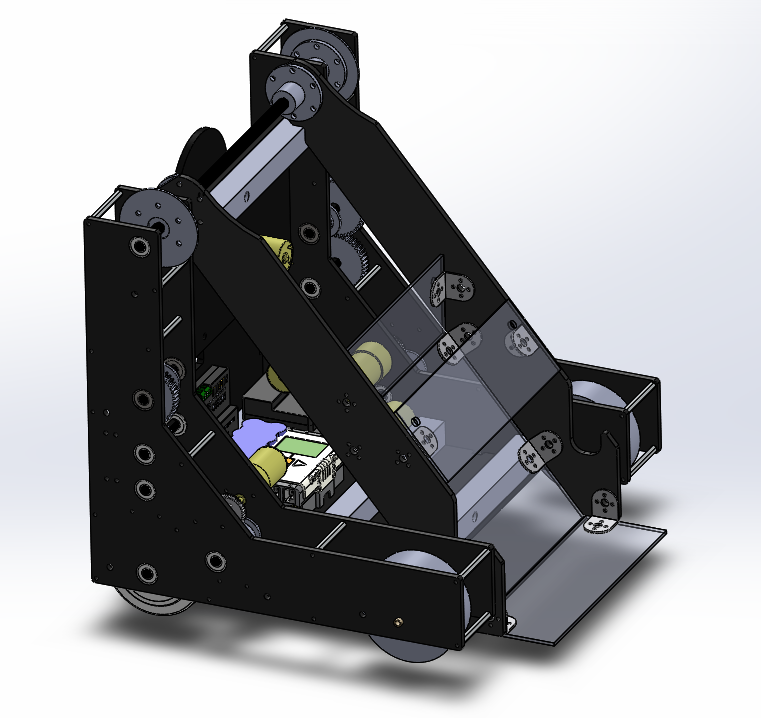
\includegraphics[scale=0.75]{images/RobotV2.png}
\end{center}
\caption{This is the second revision of our SolidWorks which includes the redesigned block acquisition device.}
\end{figure}

\newpage \subsection{First Full Test and Match -- Meeting 9: 2013-10-25}
Today was our first day having a fully complete robot. Although we had done several tests of our prototype before, this was the first day we had everything working together. The excitement within our team was immense. We tested our drive train with the added weight of the arm on the motor. We tied the flag mechanism with nylon as our Kevlar rope has not yet been received. The Kevlar provides less friction and is more like the competition.

Near the bottom, we have a lot of empty space to place the electronics. We hope to use the HiTechnic SuperPro this year to do much more sensor fusion. We want to add an Arduino or Atmel processor (ATUC3b0128) to do much more powerful computation without having to deal with the timing issues that are imposed by using the task system in RobotC and the slow clock of the NXT. We have plans to include gyroscopes, accelerometers and ultrasonic sensors. We are also looking into developing our own infrared seeker, although we are still uncertain about the feasibility of that task. 

With the A-frame design that we have we are able to distribute all of our weight to the back of the robot. This makes it very stable and very difficult to push us. 

When we scored our first block, the entire team was ecstatic. We all felt relief that we were able to lift something and score our blocks. We were somewhat surprised as to how simple it was for us to score a block. It went on just by driving backwards and raising the arm.

The arm went up very smoothly and we had no issues scoring on any of the blocks. We decided to play our first match to see how many points we were able to score.

We gave Tristan the controller and on our first run we were able to score about 200 points. We scored only on the outside baskets. This added up to the balanced bonus bonuses. Overall, we are very happy with the current design of the robot. Although, we do feel that a lot of driver practice is needed, along with an improved block acquisition device. 

Once we had the entire robot built we started testing the arm mechanism and it's ability to remove and score blocks. We found that although it is just in and out straight, moving linearly. We also found that it requires almost no effort to manipulate.

Tristan, our driver, says that with the new Fishtail drive train that we incorporated along with the ease of use of scoring blocks and removing them from the ground. We are still unable to consistently pickup 4 blocks. 

There is an air of reminiscence from our first year of FTC. We feel that our strategy and simplicity of our mechanism is very similar. This brings back memories to the members who were on the team from the conception of the team. This also brings an air of confidence among the members about the ability of our robot.

Now there is a lot of talk among the team members about autonomous and strategies for approaching it. We have the ability to determine which column the Infrared beacon is one within one second of our robot starting up.

After we scored our first block and played our first game we decided that we had accomplished a decent amount for this extra Sunday meeting and decided to call it a day. We have high hopes for the competition and expect to place well at our first qualifier. 

\newpage \subsection{Short Design Meeting -- Meeting 10: 2013-11-2}
Today was mostly a day for driver practice and minor repairs. We did several hours of practice, then moved the grabbing mechanism down an inch because it was barely outside the sizing box. This created a couple functionality issues, which will be resolved in the next meeting. We also tested the autonomous accelerometer and gyroscope, but didn't get much farther than measuring the (mostly insignificant) error before we had to leave. 

Today was short.

\newpage \subsection{Tweaking and Autonomous Programming -- Meeting 11: 2013-11-8}
Today several mechanical changes were made. The flat block grabber was moved down more, but the attached aligning bars were kept in the same place. The bars were also melted into a curve to stop the blocks from catching on them, but at the same time keeping them from falling out. In addition, we made our hex arm shafts, designed after the AndyMark hex wheel shaft. We used a lathe to create the same shape and then used a hex broach of 3/8'' to allow it to slide over. 

Another notable change was somewhat small, but it was entirely necessary. We added a funnel like system onto our arm to stop blocks from flying out as we tried to score. This was done with two small bent Tetrix pieces that redirect the blocks into the center of our scoring mechanism. 

After implementing this, the amount of blocks that we missed dropped from almost $50\%$ to nearly $2\%$. This worked phenomenally and outdid all of our expectations. 

Today was a rather complex code day. Yousuf and Kian woke up early to start work at 7 AM on autonomous. Other team members were arriving past 10. Our progress was significant and extensive, leading us into a few minor problems but also into several solutions. 

We decided immediately to write the code again from the bottom up, testing each component as we added it. The old code would have taken too long to get working properly. We struggled for around half an hour with a few simple glitches. We had a very silly error where RobotC simply refused to function properly. The eventual solution was ridiculous: the line of code with the error was replaced via copy and paste with a duplicate line from an old code file. This resolved the issue. 

Accelerometric integration now works, and we can properly integrate our position with very little noise and error. There are no issues here. 

The gyroscope integration, on the other hand, is returning garbage output. It's moderately representative of our actual rotation, but in actuality it is totally useless. The tolerance is +/- 10 degrees. I surmise this is a tasking issue, and $\delta t$ is not being set properly, resulting in error. 

We attached the infrared seeker sensors, and can now start the game consistently knowing which column the tag is in. We have a 540 degree field of view, since the two sensors face opposite directions. As such, our first movement command is to go directly to the column with the IR beacon. We may need to redesign our autonomous though since we are getting a lot of noise. 

Our plan is to turn perpendicular to the pendulum. Everything except the gyroscope is functional.

\newpage \subsection{Autonomous Working (No IR) -- Meeting 12: 2013-11-10}
This weekend, we successfully programmed our autonomous. The code allows the robot to deposit the autonomous block in any basket, as selected by the user interface. The logic for this decision works as follows:
\begin{itemize}
\item The user selects which row they would like the block placed in, if the IR beacon is in each column.
\item The robot uses triangulation with two outward-facing IR seekers to start the game immediately knowing which column contains the beacon. (This still doesn't work yet)
\item The robot angles to the correct basket.
\item The robot moves and rotates, aligning itself to score with the block.
\item The robot raises the arm, scoring the block.
\item It then backs off to move onto the ramp.
\end{itemize}

The program for this has been written, and works with an (approximated) 90\% consistency.

\newpage \subsection{Driver Practice and Lifting Locking -- Meeting 13: 2013-11-17}
The plan for the meeting was to spend an hour or two testing the autonomous for consistency at getting on top of the ramp. Then the plan was to do driver practice for the rest of the day.

Early tests of the autonomous showed some problems getting on top of the board, with the placement of the sensor being off about 30\% of the time. The most common issue occurred when the IR mounting was off center. This caused us major error. After mounting the beacon much more securely, the autonomous became very consistent at getting to the pendulum, scoring the vast majority of the time in several trials.

As we began driver practice, however, some structural problems were discovered. The cross bars that we were using to brace our lift torqued during one run, causing us concern when lifting. Tristan volunteered to create the crossbars in SolidWorks and spent some time taking careful measurements of the spacing between the two halves of the lift. The other major fix that was incorporated was to add two points of contact on each side in order to stop the arm from torquing under major force.

We also developed a lifting locking mechanism which works by jamming a third gear into our system. This induces a lock that cannot be broken and does not need power. Figure \ref{locking} shows this system in action.

\begin{figure}[H]
\begin{center}
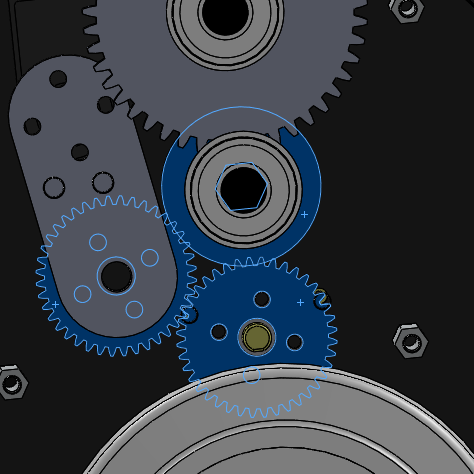
\includegraphics[scale=0.75]{images/Gearlock.png}
\end{center}
\caption{The blue sections highlighted show the three gears that are all locked together. It restricts any movement and works effectively.}
\label{locking}
\end{figure}

\newpage \subsection{Outreach -- Meeting 14: 2013-11-29}
This year we decided to mentor an FLL team and we mentored two FLL teams. We helped them program the new EV3 and taught them some new design techniques for the attachments that they had on their robot. We spent about 4 hours running through all of the programs they had and suggesting different ways that they could go about it. We also taught them how to use sensors as a lot of their programs were unreliable. We hope to start an FTC team with these students in the upcoming years. The FLL team we mentored just won their qualifier competition and has a regional competition at LegoLand on December 7th. 

\newpage \subsection{Driver Practice -- Meeting 15: 2013-12-6}
Today we mainly tested our robots abilities using time trials.  Our robot managed to pick up two to three blocks per trip, which was below our expectations.  Because of this we began experimenting with different methods of collecting blocks, such as a horizontal roller. The first material being a sheet of extremely thin sheet metal which was low enough to the ground but it was too weak, When we tried to pick up blocks the metal would buckle and make a wall impossible for anymore blocks to get up.  Our next solution was to use a thicker, flexible sheet of plastic that slid with really low friction across the ground.  The plastic sheet was just the right height to where it would fit perfectly under all of the blocks without getting deformed. 

Our next task was to be able to fit three or four blocks, no more no less.  The way we solved this greatly important problem was by using a metal deterrent to block more than five blocks from being collected.  The combination of the ramp and the deterrent made it so that we extremely rarely picked up two blocks but we also very rarely picked up more than four blocks.

Overall, we are currently scoring approximately 300 points alone per round. We hope that our speed will be unmatched and we will be able to score many points. 